\documentclass{scrartcl}
\usepackage[utf8]{inputenc}
\usepackage[english]{babel}
\usepackage[T1]{fontenc}

\parindent 0pt
\parskip 0.5em

\title{Assignment 4}
\author{Jakob Wittmann\\Dominik Schmidt}
\date{\today}

\usepackage{hyperref}
\usepackage[all]{hypcap}
\hypersetup{pdfborder = {0 0 0}, colorlinks=true, allcolors=black, urlcolor=blue}
\usepackage[margin=2.5cm]{geometry}
\usepackage{booktabs}
\usepackage{array}
\setlength{\tabcolsep}{.3em}

\usepackage{float}
\usepackage[export]{adjustbox}
\usepackage{amsmath}
\def\dd{\mathrm{d}}

\begin{document}
\maketitle
\begin{tabular}{rccccccccccccccccccc}
	\toprule
 & v1 & v2 & v3 & v4 & v5 & v6 & v7 & v8 & v9 & v10 & v11 & v12 & v13 & v14 & v15 & b1 & b2 & b3 & b4\\
	\midrule
g6p & -1 &  &  &  & -1 &  &  &  &  &  &  &  &  &  &  & 1 &  &  & \\
nadp & -1 &  &  & -1 &  &  &  &  &  &  &  &  &  &  &  &  &  &  & \\
6pgl & 1 &  & -1 &  &  &  &  &  &  &  &  &  &  &  &  &  &  &  & \\
nadph & 1 &  &  & 1 &  &  &  &  &  &  &  &  &  &  &  &  &  &  & \\
h & 1 &  &  & 1 &  &  &  &  &  &  &  &  &  &  &  &  &  &  & \\
h2o &  &  & -1 &  &  &  &  & -1 &  &  &  &  &  &  &  &  &  &  & \\
6pgc &  &  & 1 & -1 &  &  &  &  &  &  &  &  &  &  &  &  &  &  & \\
ru5p\_\_D &  &  &  & 1 &  &  & 1 &  &  &  &  & 1 &  & -1 & 1 &  &  &  & \\
co2 &  &  &  & 1 &  &  &  &  &  &  &  &  &  &  &  &  &  &  & \\
f6p &  &  &  &  & 1 & 1 &  & 1 & -1 & -1 &  &  & 1 &  &  &  &  &  & 1\\
ah6p\_\_D &  &  &  &  &  & -1 & -1 &  &  &  &  &  &  &  &  &  &  &  & \\
fald &  &  &  &  &  &  & 1 &  &  &  &  &  &  &  &  &  &  &  & \\
fdp &  &  &  &  &  &  &  & -1 & 1 & 1 & -1 &  &  &  &  &  &  &  & \\
pi &  &  &  &  &  &  &  & 1 &  &  &  &  &  &  &  &  &  &  & \\
atp &  &  &  &  &  &  &  &  & -1 &  &  &  &  &  &  &  &  &  & \\
adp &  &  &  &  &  &  &  &  & 1 & -1 &  &  &  &  &  &  &  &  & \\
amp &  &  &  &  &  &  &  &  &  & 1 &  &  &  &  &  &  &  &  & \\
dhap &  &  &  &  &  &  &  &  &  &  & 1 &  &  &  &  &  &  &  & \\
g3p &  &  &  &  &  &  &  &  &  &  & 1 & -1 & -1 &  &  &  &  & 1 & \\
s7p &  &  &  &  &  &  &  &  &  &  &  & -1 & -1 &  &  &  &  &  & \\
r5p &  &  &  &  &  &  &  &  &  &  &  & 1 &  &  & -1 &  & -1 &  & \\
xu5p\_\_D &  &  &  &  &  &  &  &  &  &  &  & 1 &  & 1 &  &  &  &  & \\
e4p &  &  &  &  &  &  &  &  &  &  &  &  & 1 &  &  &  &  &  & \\
	\bottomrule
\end{tabular}
	\clearpage
	\section{Metabolite Pathway}
		\begin{figure}[H]
			\centering
			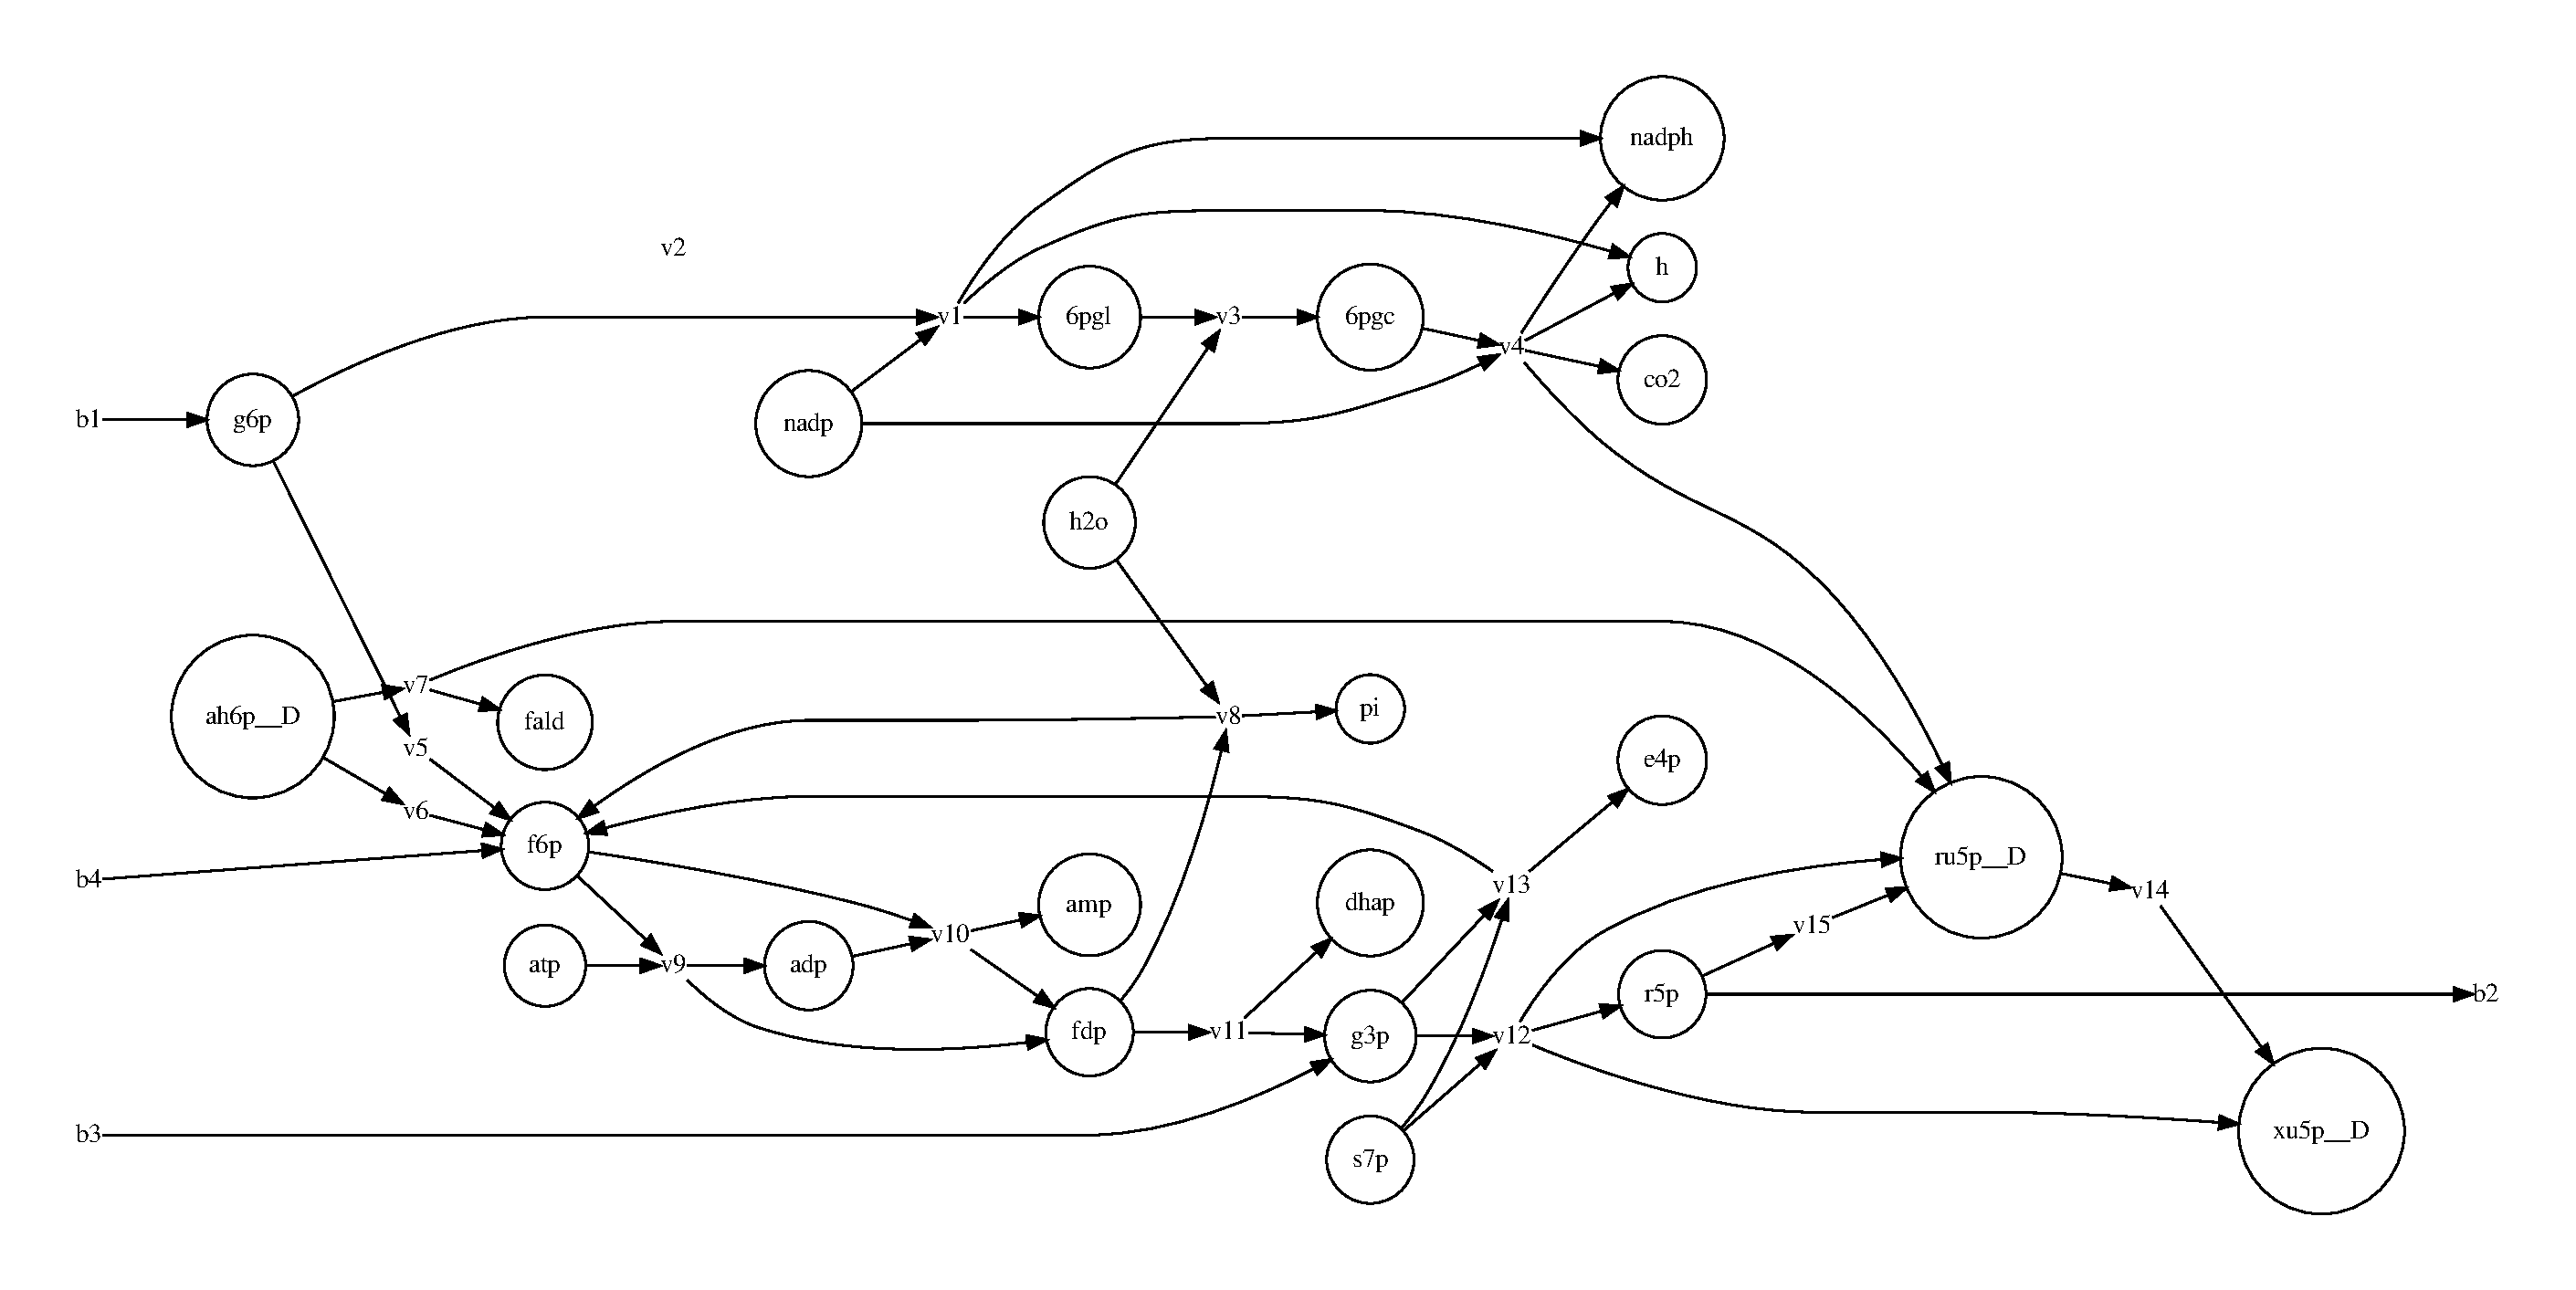
\includegraphics[max height=\linewidth, max width=0.75\paperheight, rotate=-90]{pathway.pdf}
			\caption{The metabolic pathway}
		\end{figure}
	\section{Metabolic Maps}
			\begin{minipage}{0.33\linewidth}
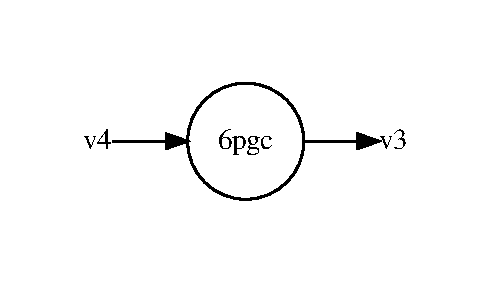
\includegraphics[max width=\linewidth]{metabolic_maps/6pgc.pdf}
\end{minipage}
\begin{minipage}{0.33\linewidth}
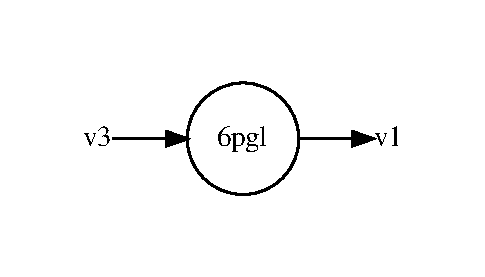
\includegraphics[max width=\linewidth]{metabolic_maps/6pgl.pdf}
\end{minipage}
\begin{minipage}{0.33\linewidth}
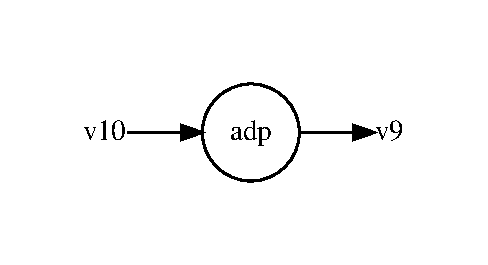
\includegraphics[max width=\linewidth]{metabolic_maps/adp.pdf}
\end{minipage}
\begin{minipage}{0.33\linewidth}
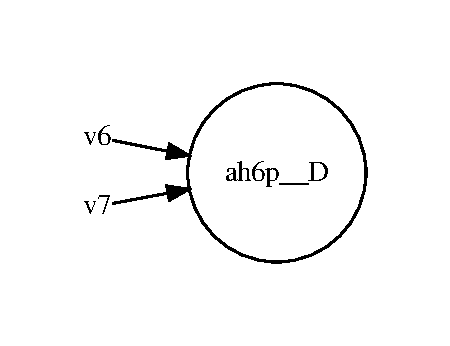
\includegraphics[max width=\linewidth]{metabolic_maps/ah6p__D.pdf}
\end{minipage}
\begin{minipage}{0.33\linewidth}
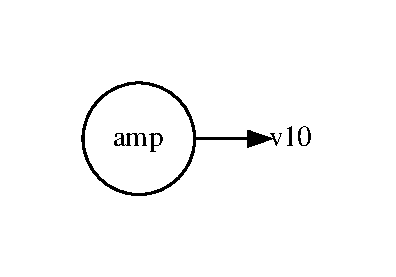
\includegraphics[max width=\linewidth]{metabolic_maps/amp.pdf}
\end{minipage}
\begin{minipage}{0.33\linewidth}
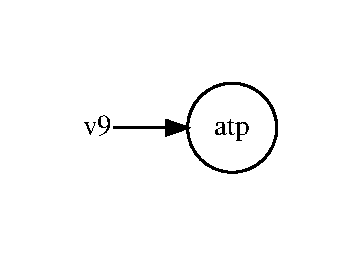
\includegraphics[max width=\linewidth]{metabolic_maps/atp.pdf}
\end{minipage}
\begin{minipage}{0.33\linewidth}
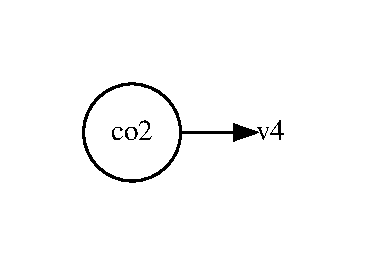
\includegraphics[max width=\linewidth]{metabolic_maps/co2.pdf}
\end{minipage}
\begin{minipage}{0.33\linewidth}
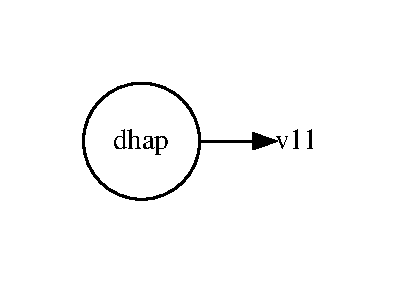
\includegraphics[max width=\linewidth]{metabolic_maps/dhap.pdf}
\end{minipage}
\begin{minipage}{0.33\linewidth}
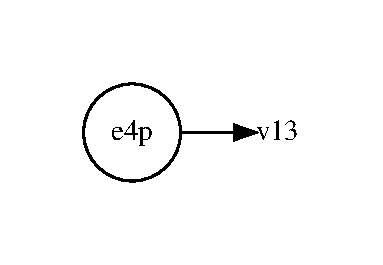
\includegraphics[max width=\linewidth]{metabolic_maps/e4p.pdf}
\end{minipage}
\begin{minipage}{0.33\linewidth}
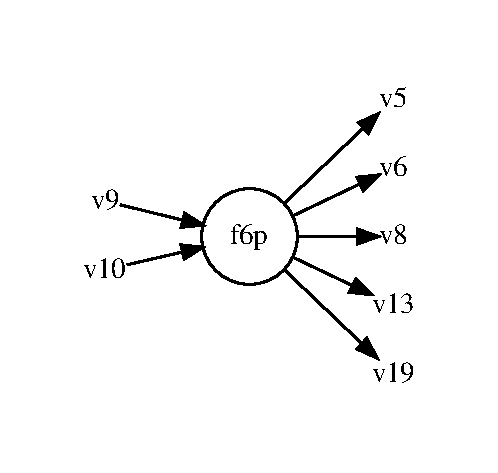
\includegraphics[max width=\linewidth]{metabolic_maps/f6p.pdf}
\end{minipage}
\begin{minipage}{0.33\linewidth}
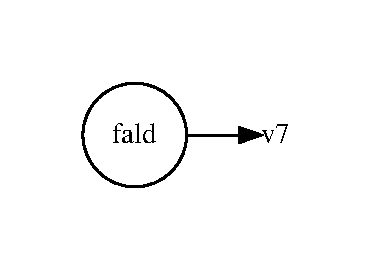
\includegraphics[max width=\linewidth]{metabolic_maps/fald.pdf}
\end{minipage}
\begin{minipage}{0.33\linewidth}
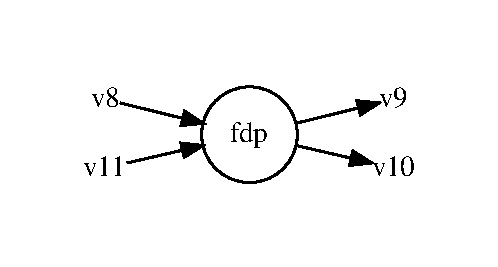
\includegraphics[max width=\linewidth]{metabolic_maps/fdp.pdf}
\end{minipage}
\begin{minipage}{0.33\linewidth}
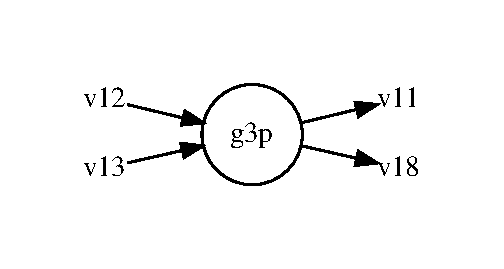
\includegraphics[max width=\linewidth]{metabolic_maps/g3p.pdf}
\end{minipage}
\begin{minipage}{0.33\linewidth}
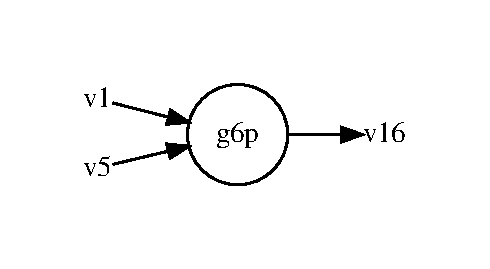
\includegraphics[max width=\linewidth]{metabolic_maps/g6p.pdf}
\end{minipage}
\begin{minipage}{0.33\linewidth}
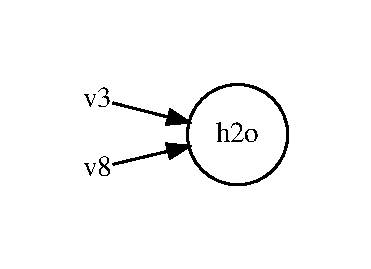
\includegraphics[max width=\linewidth]{metabolic_maps/h2o.pdf}
\end{minipage}
\begin{minipage}{0.33\linewidth}
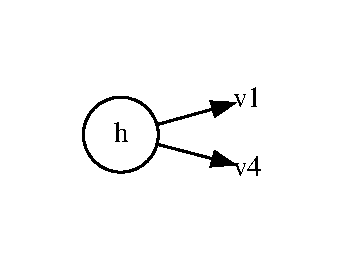
\includegraphics[max width=\linewidth]{metabolic_maps/h.pdf}
\end{minipage}
\begin{minipage}{0.33\linewidth}
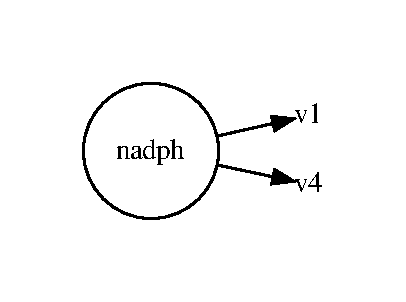
\includegraphics[max width=\linewidth]{metabolic_maps/nadph.pdf}
\end{minipage}
\begin{minipage}{0.33\linewidth}
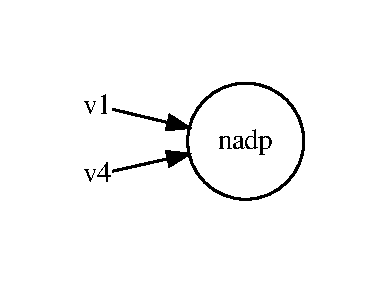
\includegraphics[max width=\linewidth]{metabolic_maps/nadp.pdf}
\end{minipage}
\begin{minipage}{0.33\linewidth}
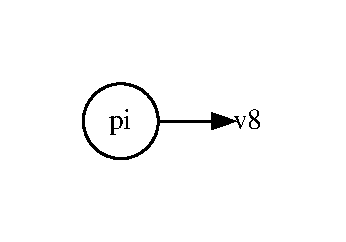
\includegraphics[max width=\linewidth]{metabolic_maps/pi.pdf}
\end{minipage}
\begin{minipage}{0.33\linewidth}
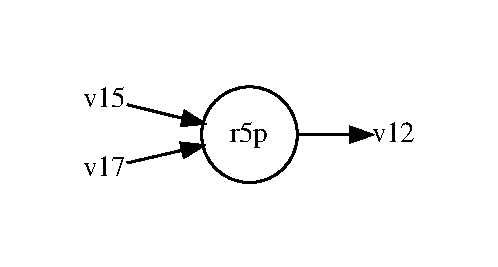
\includegraphics[max width=\linewidth]{metabolic_maps/r5p.pdf}
\end{minipage}
\begin{minipage}{0.33\linewidth}
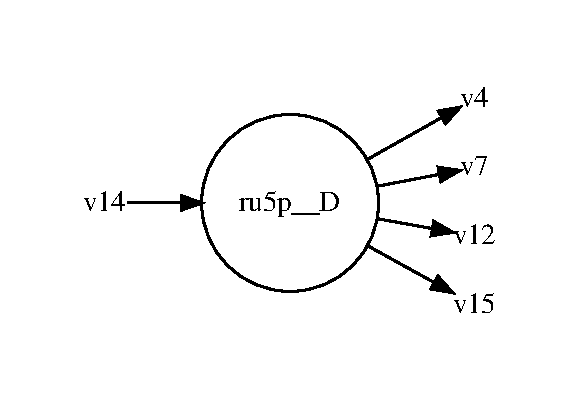
\includegraphics[max width=\linewidth]{metabolic_maps/ru5p__D.pdf}
\end{minipage}
\begin{minipage}{0.33\linewidth}
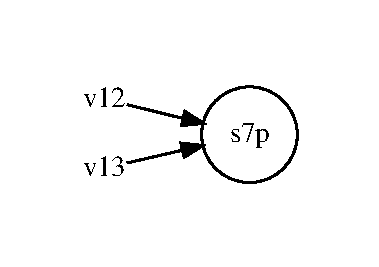
\includegraphics[max width=\linewidth]{metabolic_maps/s7p.pdf}
\end{minipage}
\begin{minipage}{0.33\linewidth}
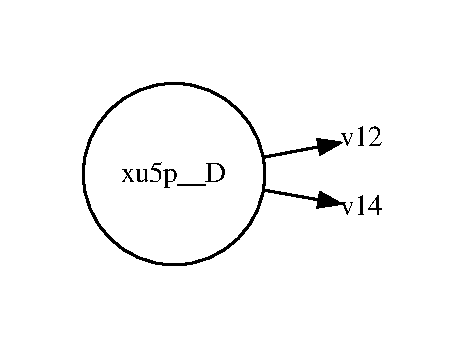
\includegraphics[max width=\linewidth]{metabolic_maps/xu5p__D.pdf}
\end{minipage}
\section{Mass Balance Equations}
\begin{align}
\frac{\dd \mathrm{g6p}}{\dd t} &=  -v1 -v5 +b1\\
\frac{\dd \mathrm{nadp}}{\dd t} &=  -v1 -v4\\
\frac{\dd \mathrm{6pgl}}{\dd t} &= v1 -v3\\
\frac{\dd \mathrm{nadph}}{\dd t} &= v1 +v4\\
\frac{\dd \mathrm{h}}{\dd t} &= v1 +v4\\
\frac{\dd \mathrm{h2o}}{\dd t} &=  -v3 -v8\\
\frac{\dd \mathrm{6pgc}}{\dd t} &= v3 -v4\\
\frac{\dd \mathrm{ru5p\_\_D}}{\dd t} &= v4 +v7 +v12 -v14 +v15\\
\frac{\dd \mathrm{co2}}{\dd t} &= v4\\
\frac{\dd \mathrm{f6p}}{\dd t} &= v5 +v6 +v8 -v9 -v10 +v13 +b4\\
\frac{\dd \mathrm{ah6p\_\_D}}{\dd t} &=  -v6 -v7\\
\frac{\dd \mathrm{fald}}{\dd t} &= v7\\
\frac{\dd \mathrm{fdp}}{\dd t} &=  -v8 +v9 +v10 -v11\\
\frac{\dd \mathrm{pi}}{\dd t} &= v8\\
\frac{\dd \mathrm{atp}}{\dd t} &=  -v9\\
\frac{\dd \mathrm{adp}}{\dd t} &= v9 -v10\\
\frac{\dd \mathrm{amp}}{\dd t} &= v10\\
\frac{\dd \mathrm{dhap}}{\dd t} &= v11\\
\frac{\dd \mathrm{g3p}}{\dd t} &= v11 -v12 -v13 +b3\\
\frac{\dd \mathrm{s7p}}{\dd t} &=  -v12 -v13\\
\frac{\dd \mathrm{r5p}}{\dd t} &= v12 -v15 -b2\\
\frac{\dd \mathrm{xu5p\_\_D}}{\dd t} &= v12 +v14\\
\frac{\dd \mathrm{e4p}}{\dd t} &= v13\\
\end{align}
\end{document}
